\documentclass{article}
\usepackage{esc103}

\title{ESC103: Exam Review}
\author{QiLin Xue}
\date{Fall 2020}
\usepackage{lmodern}
\usepackage{tikz}
\usepackage{pgfplots}
\usepackage{bm}
\usepackage{textcomp}
\usepackage{graphicx}
\usepackage{bbm}
\usepackage{parskip}
\usepackage{multicol}
\makeatletter
\renewcommand*\env@matrix[1][*\c@MaxMatrixCols c]{%
  \hskip -\arraycolsep
  \let\@ifnextchar\new@ifnextchar
  \array{#1}}
\makeatother
\usetikzlibrary{arrows}
\pgfplotsset{compat=1.16}
\setlength\parindent{0pt}
\everymath{\displaystyle}
\usepackage{makeidx}
\makeindex
\let\oldtextbf\textbf
\renewcommand{\textbf}[1]{\oldtextbf{#1}\index{#1}}


\usepackage{xstring}
\usepackage{forloop}


\begin{document}
\newcounter{idx}
\newcounter{posx}
\newcommand{\rotraise}[1]{%
  \StrLen{#1}[\slen]
  \forloop[-1]{idx}{\slen}{\value{idx}>0}{%
    \StrChar{#1}{\value{idx}}[\crtLetter]%
    \IfSubStr{tlQWERTZUIOPLKJHGFDSAYXCVBNM}{\crtLetter}
      {\raisebox{\depth}{\rotatebox{180}{\crtLetter}}}
      {\raisebox{1ex}{\rotatebox{180}{\crtLetter}}}}%
}

\maketitle
Please let me know via discord (Qcumber\#4444) if I am missing anything, there exists any typos, and especially if something is horrendously wrong! Note that this is an unofficial resource and I am not responsible if the use of this study sheet causes you to fail the exam, break up with your partner, find your house burned down, or be captured by the North Korean government to be forced to work on their nuclear missile project which leads to the destruction of the entire world.
\tableofcontents
\printindex
\newpage
\section{Basic Vectors}
The \textbf{linear combination} of vectors $\vec{v}$ and $\vec{w}$ is given by:
\begin{equation}
    c\vec{v}+d\vec{w}
    \label{eq:}
\end{equation}
where $c$ and $d$ are scalars. Note that \textbf{vector addition} is both \textbf{associative} and \textbf{commutative.}

The length of a vector in $\vec{v}$ in $\mathbb{R}^N$ is given by:
\begin{equation}
    \lVert v\rVert = \sqrt{v_1^2+v_2^2+\cdots+V_N^2}
    \label{eq:}
\end{equation}
The \textbf{dot product} (also known as scalar product) is defined as:
\begin{equation}
    \vec{v}\cdot\vec{w} = v_1w_1+v_2w_2+v_3w_3+\cdots+v_Nw_N
    \label{eq:}
\end{equation}
for two vectors $\vec{v}$ and $\vec{w}$ in $\mathbb{R}^N$. Using these, we can derive the following ideas and theorems.
\begin{idea}
    The dot product of a vector with itself gives the square of its length:
    \begin{equation}
        \lVert \vec{v}\rVert ^2 = \vec{v}\cdot \vec{v}
        \label{eq:}
    \end{equation}
\end{idea}
\begin{idea}
    The \textbf{angle between two vectors} is given by:
    \begin{equation}
        \cos\theta = \frac{\vec{w}\cdot\vec{v}}{\lVert \vec{w}\rVert \lVert \vec{v} \rVert}
    \end{equation}
\end{idea}
\begin{idea}
    The \textbf{triangle inequality} is:
    \begin{equation}
        \lVert \vec{v}+\vec{w} \rVert \le \lVert\vec{v}\rVert + \lVert\vec{v}\rVert
        \label{eq:}
    \end{equation}
\end{idea}
\begin{idea}
    The \textbf{Cauchy-Schwarz-Bunakowsky Inequality} is:
    \begin{equation}
        |\vec{v}\cdot\vec{w}| \le \lVert\vec{v}\rVert \lVert\vec{w}\rVert
        \label{eq:}
    \end{equation}
\end{idea}
\begin{idea}
    The \textbf{projection} of $\vec{w}$ on $\vec{v}$ can be written as:
    \begin{equation}
        \vec{u}=\text{proj}_{\vec{v}}\vec{w}=\frac{\vec{w}\cdot\vec{v}}{\lVert \vec{v} \rVert^2}\vec{v} = \frac{\vec{w}\cdot\vec{v}}{\lVert\vec{v}\rVert}\frac{\vec{v}}{\lVert\vec{v}\rVert}
        \label{eq:}
    \end{equation}
    You can view the last part $\frac{\vec{v}}{\lVert \vec{v}\rVert}$ as a unit vector pointing in the direction of $\vec{v}$ such that the \textbf{scalar projection} can be defined as:
    \begin{equation}
        |\vec{u}| = |\text{proj}_{\vec{v}}\vec{w}| = \left|\frac{\vec{w}\cdot\vec{v}}{\lVert \vec{v}\rVert}\right|
        \label{eq:}
    \end{equation}
\end{idea}
\section{Plane Geometry}
The \textbf{cross product} is defined as:
\begin{equation}
    \vec{u}=\vec{v}\times \vec{w}=
    \begin{bmatrix}
        v_2w_3-v_3w_2 \\ 
        v_3w_1-v_1w_3 \\ 
        v_1w_2-v_2w_1
    \end{bmatrix}
\end{equation}
which has a magnitude of $\lVert \vec{u}\times\vec{w}\rVert = \lVert \vec{u}\rVert \lVert \vec{w}\rVert \sin\theta$. The direction can be determined using the \textbf{right hand rule}. Cross products have the following properties:
\begin{property}
    The properties of a cross product is as follows.
    \begin{itemize}
        \item Consider $3$ vectors, $\vec{v}$, $\vec{w}$, and $\vec{z}$. Then:
        \begin{equation}
            \vec{v}\times (\vec{w}+\vec{z}) = \vec{v} \times \vec{w} + \vec{v} \times \vec{z}
            \label{eq:}
        \end{equation}
        \item The cross product is not commutative, but they are \textbf{anti-commutative}:
        \begin{equation}
            \vec{v}\times \vec{w} = -\vec{w}\times \vec{v}
            \label{eq:}
        \end{equation}
        \item When crossed with the zero vector, we have:
        \begin{equation}
            \vec{v}\times \vec{0} = \vec{0}\times \vec{v} = \vec{0}
            \label{eq:}
        \end{equation}
        \item When multiplied by a scalar,
        \begin{equation}
            c(\vec{v}\times\vec{w}) = (c\vec{v})\times \vec{w} = \vec{v}\times (c\vec{w})
            \label{eq:}
        \end{equation}
    \end{itemize}
\end{property}
\begin{idea}
    The magnitude of the cross product between $\vec{v}$ and $\vec{w}$ gives the area of a parallelogram made by $\vec{v}$ and $\vec{w}$.
\end{idea}
We can write out any point on a plane given a linear combination of two vectors $\vec{d}_1$ and $\vec{d}_2$ which span the plane:
\begin{equation}
    \begin{bmatrix}
        x\\y\\z
    \end{bmatrix}=\begin{bmatrix}
        x_0\\y_0\\z_0
    \end{bmatrix}+c\vec{d}_1+d\vec{d}_2
    \label{eq:}
\end{equation}
where $\begin{bmatrix}
    x_0\\y_0\\z_0
\end{bmatrix}$ is any known point on the plane. Additionally, we can define a plane by its normal vector:
\begin{equation}
    \vec{n}=\begin{bmatrix}
        a\\b\\c
    \end{bmatrix}
    \label{eq:}
\end{equation}
by taking the cross product between any two vectors $\overrightarrow{P_0P}$ that lie on the plane such that:
\begin{equation}
    \overrightarrow{P_0P} \cdot \vec{n} = 0
    \label{eq:}
\end{equation}
Using this information, we can derive the following theorems and ideas:
\begin{idea}
    If $\vec{n}=\begin{bmatrix}
        a\\b\\c
    \end{bmatrix}$ is a normal vector, then the plane that it defines can be represented by the \textbf{scalar equation} $ax+by+cz+d=0$.
    \begin{proof}
        Suppose we know a given point $P_0=\begin{bmatrix}
            x_0\\y_0\\z_0
        \end{bmatrix}$ on the plane. Then we can choose any other point on the plane $P=\begin{bmatrix}
            x\\y\\z
        \end{bmatrix}$ which can define any arbitrary vector that is paralell to the plane:
        \begin{equation}
            \vec{v} = P-P_0 = \begin{bmatrix}
                x-x_0\\y-y_0\\z-z_0
            \end{bmatrix}
            \label{eq:}
        \end{equation}
        The dot product between $\vec{v}$ and $\vec{n}$ must be equal to zero, which gives:
        \begin{equation}
            a(x-x_0)+b(y-y_0)+c(z-z_0)=0
            \label{eq:}
        \end{equation}
        Expanding, we get the form that we desire.
    \end{proof}
\end{idea}
\begin{idea}
    The distance from a point $P=(x_0,y_0,z_0)$ to the plane $ax+by+cz+d=0$ is given by:
    \begin{equation}
        D = \frac{|ax_0+by_0+cz_0+d|}{\sqrt{a^2+b^2+c^2}}
        \label{eq:}
    \end{equation}
    \textit{Note:} We are not allowed to use this formula on the test, but we can derive it below. Refer to the following diagram:
\begin{center}
    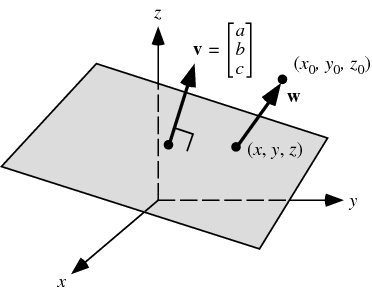
\includegraphics[width=0.4\linewidth]{plane-point.png}
\end{center}
    \begin{proof}
        The normal vector to the plane is given by:
        \begin{equation}
            \vec{n}=\begin{bmatrix}
                a\\b\\c
            \end{bmatrix}
            \label{eq:}
        \end{equation}
        
        Define $\vec{w}$ as the vector from any point $P$ to any given point $(x,y,z)$ on the plane such that:
        \begin{equation}
            \vec{w} = \begin{bmatrix}
                x-x_0\\ 
                y-y_0 \\ 
                z-z_0
            \end{bmatrix}
            \label{eq:}
        \end{equation}
        The scalar projection of $\vec{w}$ on $\vec{n}$ then gives the orthogonal component, and thus the shortest distance between $P$ and the plane:
        \begin{align}
            D &= |\text{proj}_{\vec{n}}\vec{w}| \\ 
            &= \frac{|\vec{n}\cdot\vec{w}|}{|\vec{v}|} \\ 
            &=
             \left|\frac{a(x-x_0)+b(y-y_0)+c(z-z_0)}{\sqrt{a^2+b^2+c^2}}\right| \\ 
             &= \left|\frac{(ax+by+cz)-ax_0-by_0-cz_0}{\sqrt{a^2+b^2+c^2}}\right| \\ 
             &= \left|\frac{-d-ax_0-by_0-cz_0}{\sqrt{a^2+b^2+c^2}}\right| \\ 
             &= \left|\frac{d+ax_0+by_0+cz_0}{\sqrt{a^2+b^2+c^2}}\right|
        \end{align}
    \end{proof}
    This is the general way when determining the distance from a point to a plane. You first need to figure out the normal vector (e.g. this can also be done by determining two vectors that lie parallel to the plane and taking their cross product), and then the vector between any given point to the point of interest. Getting the orthogonal projection yields the distance to the plane.
\end{idea}
\begin{idea}
    The projection of a vector $\vec{v}$ onto a plane $\Pi$ defined by the normal vector $\vec{n}$ is:
    \begin{equation}
        \text{proj}_{\Pi} = \vec{v}-\text{proj}_{\vec{n}}\vec{v}
        \label{eq:}
    \end{equation}
    We can also show this by drawing a picture!
\end{idea}
\section{Matrix Multiplication and Linear Transformations}
A matrix can be used to represent systems of linear equations. For example, the following set:
\begin{align}
    x-2y&=1 \\ 
    3x+2y&=11
\end{align}
can be represented by a \textbf{row picture}, which represents the classical ``find the intersection'' visual approach. It can also be represented via a \textbf{column picture}:
\begin{equation}
    x\begin{bmatrix}
        1\\3
    \end{bmatrix}
    +y\begin{bmatrix}
    -2\\2
    \end{bmatrix}=\begin{bmatrix}
        1\\11
    \end{bmatrix}
    \label{eq:}
\end{equation}
It can also be represented via matrices:
\begin{equation}
    \underbrace{\begin{bmatrix}
        1&-2\\3&2
    \end{bmatrix}}_\text{Matrix A}\underbrace{\begin{bmatrix}
        x\\y
    \end{bmatrix}}_{\text{vector } \vec{x}}=\underbrace{\begin{bmatrix}
        1\\11
    \end{bmatrix}}_{\text{vector }\vec{b}}
\end{equation}
We can perform \textbf{matrix multiplication} if $A$ has $n$ columns and $B$ has $n$ rows.
\begin{idea}
    hen multiplying two matrices, the entry in row $i$ and column $j$ of $AB$ is:
    \begin{equation}
        \text{(Row i of A)} \cdot \text{(column j of B)}
    \end{equation}
    Recall that $A$ and $B$ can only be multiplied of $A$ is $m\times n$ and $B$ is $n\times p$. The size of the resulting matrix is therefore $m\times p$.
\end{idea}
\begin{property}
    \begin{enumerate}
        \item $A+B=B+A$ (commutative)
        \item $c(A+B)=cA+cB$ (where $c$ is scalar)
        \item $A+(B+C)=(A+B)+C$ (associative)
        \item $C(A+B)=CA+CB$ (distributive from left)
        \item $(A+B)C=AC+BC$ (distributive from right)
        \item $A(BC)=(AB)C$ (associative)
    \end{enumerate}
\end{property}
Matrices can also be viewed as \textbf{linear transformations}. $L$ represents a linear operator iff:
\begin{enumerate}
    \item $L(c\vec{v})=cL(\vec{v})$
    \item $L(\vec{v}+\vec{w})=L(\vec{v})+L(\vec{w})$
\end{enumerate}
\begin{idea}
    All linear transformations can be summarized by matrices and represented by matrix multiplication of a vector. We can determine the matrix associated with the transformation by analyzing what happens to the unit vectors $\vec{i}$, $\vec{j}$, and $\vec{k}$, under the transformation.
\end{idea}
Using the above information, we can show the following ideas:
\begin{idea}
    The \textbf{projection} of vector $\vec{w}$ on $\vec{v}$ can be written using the linear transformation $T_2$ such that:
    \begin{equation}
        \vec{u}=T_2(\vec{w}) = \frac{1}{v_1^2+v_2^2+v_3^2}\begin{bmatrix}
            v_1^2 & v_1v_2 & v_1v_3 \\ 
            v_2v_1 & v_2^2 & v_2v_3 \\ 
            v_3v_1 & v_3v_2 & v_3^2
        \end{bmatrix}\begin{bmatrix}
            w_1\\w_2\\w_3
        \end{bmatrix}
    \end{equation}
\end{idea}
\begin{idea}
    The \textbf{identity} matrix:
        \begin{equation}
            I(\vec{w})=\vec{w}
            \label{eq:}
        \end{equation}
        where:
        \begin{equation}
            I=\begin{bmatrix}
                1&0&0\\ 
                0&1&0\\ 
                0&0&1
            \end{bmatrix}
            \label{eq:}
        \end{equation}
\end{idea}
\begin{idea}
    Suppose we have a transformation $T_1$ and $T_2$, we can define a \textbf{composition} of these transformations as:
    \begin{equation}
        T_3(\vec{v})=T_2(T_1(\vec{v})) = M_{T_2}M_{T_1}\vec{v}=M_{T_3}
        \label{eq:}
    \end{equation}
    where $M$ represents the matrix associated with the linear transformations.
\end{idea}
\begin{idea}
    We want to derive the \textbf{double angle} formulas with matrix multiplication. Suppose we wish to determine the matrix associated with the transformation of rotating a vector by an angle $\theta$ counterclockwise. We think about where the $\vec{i}$ and $\vec{j}$ vectors go to, which are $\begin{bmatrix}
        \cos\theta \\ \sin\theta
    \end{bmatrix}$ and $\begin{bmatrix}
        -\sin\theta \\ \cos\theta
    \end{bmatrix}$ respectively, so the matrix associated with it is thus:
    \begin{equation}
        M_{T_\theta} = \begin{bmatrix}
            \cos\theta & -\sin\theta \\ 
            \sin\theta & \cos\theta
        \end{bmatrix}
    \end{equation}
    which is known as the \textbf{rotation} matrix. So rotating an angle by $2\theta$ is equivalent to applying the transformation $T_\theta(T_\theta(\vec{v}))$:
    \begin{equation}
        M_{T_\theta}^2 = \begin{bmatrix}
            \cos2\theta & -\sin2\theta \\ 
            \sin2\theta & \cos2\theta
        \end{bmatrix} = \begin{bmatrix}
            \cos\theta & -\sin\theta \\ 
            \sin\theta & \cos\theta
        \end{bmatrix}\begin{bmatrix}
            \cos\theta & -\sin\theta \\ 
            \sin\theta & \cos\theta
        \end{bmatrix}
        \label{eq:}
    \end{equation}
    or:
    \begin{equation}
        \begin{bmatrix}
            \cos2\theta & -\sin2\theta \\ 
            \sin2\theta & \cos2\theta
        \end{bmatrix} = \begin{bmatrix}
            \cos^2\theta-\sin^2\theta & -2\sin\theta\cos\theta \\ 
            2\sin\theta\cos\theta & \cos^2\theta-\sin^2\theta
        \end{bmatrix}
        \label{eq:}
    \end{equation}
\end{idea}
\section{Eigenvalues, Inverse, and Determinants}
The motivation behind this section is that most vectors change direction when they are multiplied by a matrix, except a few certain ones which have very special properties.
\begin{definition}
    \textbf{Eigenvectors} are special vectors associated with a certain transformation $T$ such that they don't change directions under a linear transformation. We can denote these vectors $\vec{w}$ as solutions to the linear equation (where $\vec{w}\neq \vec{0}$):
    \begin{equation}
        M\vec{w}=\lambda\vec{w}
    \end{equation}
    where the scalar $\lambda$ is the \textbf{eigenvalue} of matrix $M$.
\end{definition}
Many times, we can determine the eigenvectors and eigenvalues by drawing a picture and using intuition. In the lecture, the following matrices were used as examples:
\begin{itemize}
    \item The projection matrix. {\small (Answer: $\vec{w}$: any vector parallel or perpendicular to the projection. $\lambda$: 1 and 0 respectively.)}
    \item A reflection matrix. {\small (Answer: $\vec{w}$: any vector parallel or perpendicular to the line of reflection. $\lambda$: 1 and -1 respectively.)}
    \item A rotation matrix. {\small (Answer: None, at least in $\mathbb{R}^2$.)}
\end{itemize}
\begin{idea}
    However, sometimes intuition fails. We can solve the eigenvalue eigenvector equation as follows (this uses information from later on in this section):
\begin{align}
    M\vec{w} &= \lambda\vec{w} \\ 
    (M-I\lambda)\vec{w} &= \vec{0}
\end{align}
Since $M-I\lambda$ is not invertible, then the determinant of $M-I\lambda$ is zero, or:
\begin{equation}
    \det(M-\lambda I)=0
\end{equation}
This is the equation we need to solve to find the eigenvalue $\lambda$.
\end{idea}

Another problem in linear algebra is finding \textbf{inverses}. Suppose $\vec{u}$ and $\vec{T}$ were given and we wish to find $\vec{w}$ in the following equation:
\begin{equation}
    \vec{u}=T(\vec{w})
\end{equation}
If we can find the inverse $T^{-1}$ where $T^{-1}T=TT^{-1}=I$, then:
\begin{equation}
    \vec{w}=T^{-1}(\vec{u})
    \label{eq:}
\end{equation}
\begin{idea}
    Calculating $T^{-1}$ is equivalent to expanding $T^{-1}T$ and demanding each entry corresponds to the corresponding entry in the identity matrix. For example, if $T=\begin{bmatrix}
        a&b\\c&d
    \end{bmatrix}$ and $T^{-1}=\begin{bmatrix}
        e&f\\g&h
    \end{bmatrix}$, then:
    \begin{align}
        \begin{bmatrix}
            e&f\\g&h
        \end{bmatrix}\begin{bmatrix}
            a&b\\c&d
        \end{bmatrix} = \begin{bmatrix}
            1&0\\0&1
        \end{bmatrix}
    \end{align}
    which gives the system of four equations and four unknowns when expanded. It turns out that the inverse $T^{-1}$ is:
    \begin{equation}
        T^{-1} = \frac{1}{ad-bc}\begin{bmatrix}
            d&-b\\-c&a
        \end{bmatrix}
        \label{eq:}
    \end{equation}
\end{idea}
The quantity that we factor out $ad-bc$ is the \textbf{determinant} of the matrix, and in order for the inverse to exist, it cannot equal zero. If the inverse exists, we call it \textbf{invertible.}
\begin{definition}
    The determinant of $M=\begin{bmatrix}
        a&b\\c&d
    \end{bmatrix}$ can be written as:
    \begin{equation}
        \det(M)=ad-bc
        \label{eq:}
    \end{equation}
\end{definition}
A few other ideas that follow:
\begin{idea}
    The inverse of the projection matrix does not exist. This can be interpreted both with determinants (rigorously) and geometrically (it's an irreversible process).
\end{idea}
\begin{idea}
    In the eigenvector eigenvalue equation:
    \begin{equation}
        M\vec{v} = \lambda\vec{v}
        \label{eq:}
    \end{equation}
    the quantity $M-\lambda I$ is not invertible.
\end{idea}
% \begin{idea}
%     The eigenvalues of the matrix $M=\begin{bmatrix}
%         a&b\\c&d
%     \end{bmatrix}$ are:
%     \begin{equation}
%         \lambda = \frac{a+b}{2} \pm \sqrt{\left(\frac{a-d}{2}\right)^2+bc}
%         \label{eq:}
%     \end{equation}
% \end{idea}
\section{Gaussian Elimination}
\textbf{Gaussian Elimination} is a systematic method of solving systems of equations with an arbitrary number of variables.
Suppose we want to solve the following system:
    \begin{align}
        x+2y+z&=2\\ 
        3x+8y+z&=12\\ 
        4y+z &=2
    \end{align}
    we can write the left hand side in a much nicer form:
    \begin{equation}
        A=\begin{bmatrix}
            \boxed{1} & 2 & 1\\ 
            3 & 8 & 1 \\ 
            0 & 4 & 1
        \end{bmatrix}
        \label{eq:elimination step 1}
    \end{equation}
    and perform our classical elimination techniques but applied on the matrix. The first step is to eliminate all other numbers in the column of, and below the boxed number, known as the \textit{pivot}.
    \begin{warning}
        In computational practices, it is helpful to select a larger pivot. Selecting a small pivot can introduce a lot of error when rounding.
    \end{warning}
    \begin{equation}
        \begin{bmatrix}
        \boxed{1} & 2 & 1\\ 
        3 - 3(1) & 8 - 3(2) & 1 - 3(1) \\ 
        0 & 4 & 1
        \end{bmatrix}
        =
        \begin{bmatrix}
            \boxed{1} & 2 & 1\\ 
            0 & 2 & -2 \\ 
            0 & 4 & 1
        \end{bmatrix}
        \label{eq:elimination step 2}
    \end{equation}
    The $(2,1)$ and $(3,1)$ positions are both zero, so we can move on to the second pivot and wipe out the $(3,1)$ position.
    \begin{equation}
        \begin{bmatrix}
            \boxed{1} & 2 & 1\\ 
            0 & \boxed{2} & -2 \\ 
            0 & 4 & 1
        \end{bmatrix}
        \to 
        \begin{bmatrix}
            \boxed{1} & 2 & 1\\ 
            0 & \boxed{2} & -2 \\ 
            0 & 4-2(2) & 1-2(-2) 
        \end{bmatrix}
        =
        \begin{bmatrix}
            \boxed{1} & 2 & 1\\ 
            0 & \boxed{2} & -2 \\ 
            0 & 0 & \boxed{5} 
        \end{bmatrix}\equiv u
        \label{eq:elimination step 3}
    \end{equation}
    \begin{warning}
        The pivot chosen \textit{cannot} be equal to zero. If a pivot was originally zero (e.g. the $(1,1)$ index is zero), we will instead swap rows with a lower equation. For example, if the $(2,2)$ index is a $6$ instead of a $8$, we can swap the bottom two rows.
        \vspace{2mm}

        If there are no possible row exchanges, then it is a complete failure and it means the matrix is \textit{not invertible}
    \end{warning}
    We then perform the same operations on the right hand side:
    \begin{equation}
        b=\begin{bmatrix}
            2\\12\\2 
        \end{bmatrix}
        \to
        \begin{bmatrix}
            2\\12-3(2)\\2
        \end{bmatrix}
        \to 
        \begin{bmatrix}
            2\\6\\2-2(6)
        \end{bmatrix}
        \to 
        \begin{bmatrix}
            2\\6\\-10
        \end{bmatrix} 
        \label{eq:elimination step 4}
    \end{equation}
    We can combine both parts together in an \textbf{augmented matrix}:
    \begin{equation}
        \begin{bmatrix}[ccc|c]
            1 & 2 & 1 & 2 \\
            0 & 2 & -2 & 6 \\ 
            0 & 0 & 5 & -10
          \end{bmatrix}
    \end{equation}
    At the end of the \textbf{forward step}, the matrix satisfies three properties:
    \begin{itemize}
        \item If the first nonzero entry in row $i$ is in column $c_i$, then $i<j$ implies $c_i < c_j$. This means the first nonzero entry moves to the right as we move down the rows.
        \item The entries in the column beneath the first nonzero entry in each row are all zero.
        \item Any zero rows occur beneath all the nonzero rows.
    \end{itemize}
    In \textbf{back substitution}, we perform similar operations but in reverse order. Starting with the last nonzero row, normalize the row by its first nonzero entry:
    \begin{equation}
        \begin{bmatrix}[ccc|c]
            1 & 2 & 1 & 2 \\
            0 & 2 & -2 & 6 \\ 
            0 & 0 & 5 & -10
          \end{bmatrix} \rightarrow 
            \begin{bmatrix}[ccc|c]
                1 & 2 & 1 & 2 \\
                0 & 2 & -2 & 6 \\ 
                0 & 0 & 1 & -2
              \end{bmatrix}
    \end{equation}
    We then add multiples of this row to previous rows so that all the entires in the column containing the leading $1$ are zero:
    \begin{equation}
            \begin{bmatrix}[ccc|c]
                1 & 2 & 1-1(0) & 2-1(-2) \\
                0 & 2 & -2+2(1) & 6+2(-2) \\ 
                0 & 0 & 1 & -2
              \end{bmatrix}
              \rightarrow
              \begin{bmatrix}[ccc|c]
                1 & 2 & 0 & 4 \\
                0 & 2 & 0 & 2 \\ 
                0 & 0 & 1 & -2
              \end{bmatrix}
    \end{equation}
    We can move up the matrix and repeat:
    \begin{equation}
          \begin{bmatrix}[ccc|c]
            1 & 2 & 0 & 4 \\
            0 & 2 & 0 & 2 \\ 
            0 & 0 & 1 & -2
          \end{bmatrix} \rightarrow
          \begin{bmatrix}[ccc|c]
            1 & 2 & 0 & 4 \\
            0 & 1 & 0 & 1 \\ 
            0 & 0 & 1 & -2
          \end{bmatrix}
          \rightarrow
          \begin{bmatrix}[ccc|c]
            1 & 2-2(1) & 0 & 4-2(1) \\
            0 & 1 & 0 & 1 \\ 
            0 & 0 & 1 & -2
          \end{bmatrix}
          \rightarrow
          \begin{bmatrix}[ccc|c]
            1 & 0 & 0 & 2 \\
            0 & 1 & 0 & 1 \\ 
            0 & 0 & 1 & -2
          \end{bmatrix}
    \end{equation}
    The matrix is now in \textbf{reduced normal form.} and the solution can be easily read off as:
    \begin{equation}
        \begin{bmatrix}
            x\\y\\z
        \end{bmatrix} = \begin{bmatrix}
            2\\1\\-2
        \end{bmatrix}
        \label{eq:}
    \end{equation}
    
    \begin{warning}
        Note that occasionally, the shape of the matrix will not be a square. This is the case if \textbf{free variables} existed, which are free to take on any value they wish. For example, if the original system was instead:
        \begin{align}
            x+2y+z&=2\\ 
            3x+8y+z&=12
        \end{align}
        Then the augmented matrix in reduced normal form would instead be:
        \begin{equation}
            \begin{bmatrix}[ccc|c]
                1 & 0 & 3 & -4 \\
                0 & 1 & -1 & 3
            \end{bmatrix}
            \label{eq:}
        \end{equation}
        and the solution can be written as:
        \begin{equation}
            \begin{bmatrix}
                x\\y\\z
            \end{bmatrix} =
            \begin{bmatrix}
                -4\\3\\0 
            \end{bmatrix}
            +
            z\begin{bmatrix}
                -3 \\ 1 \\ 1
            \end{bmatrix}
            \label{eq:}
        \end{equation}
        Here, $x$ and $y$ are leading variables while $z$ is a free variable. Check that this leads to the same outcome as above when $z=-2$.
    \end{warning}
    \begin{idea}
        In general, the reason Gaussian Elimination works is because \textbf{elementary row operations} do not change the system of equations. These include:
        \begin{enumerate}
            \item Interchanging the rows
            \item Multiplying one row by a nonzero constant
            \item Adding or subtracting a multiple of one row to or from another row
        \end{enumerate}
    \end{idea}
    \subsection{Rank}
    A system consisting of $m$ equations and $n$ unknowns produces a $m\times n$ coefficient matrix $A$, where:
    \begin{equation}
        A\vec{x} = \vec{b}
        \label{eq:}
    \end{equation}
    However, $m\times n$ is not necessarily the true size of the system as equations, which can occur in the following cases:
    \begin{itemize}
        \item If a redundant equation like $0=0$ appears.
        \item If there are two identical rows.
        \item If one row is a combination of two other rows.
    \end{itemize}
    \begin{definition}
        If the reduced normal form (RNF) of matrix $A$ is unique, then the number of leading ones in the RNF is the RNF of matrix $A$ is called the \textbf{rank} of matrix $A$ and is denoted as:
        \begin{equation}
            r = \text{rank}(A)
            \label{eq:}
        \end{equation}
        The true size of matrix $A$ is given by its rank.
    \end{definition}
    There are three general outcomes that arise from solving a system of equations:
    \begin{enumerate}
        \item A unique solution: occurs when ever variable in the reduced normal form is a leading variable. This is represented by:
        $
            r=m=n
        $ and is only valid for a square matrix.
        \item Infinite solutions: occurs when there is at least one free variable in reduced normal form. 
        \item No solution: occurs when we get a row like:
        \begin{equation}
            \begin{bmatrix}[ccccc|c]
                0&0&0&\cdots&0&a
            \end{bmatrix}
            \label{eq:}
        \end{equation}
        at any point during the elimination, with $a\neq 0$.
    \end{enumerate}
    There are a few \textbf{non-square} systems you should be familiar with. For \textbf{tall and thin} systems such as the following $3 \times 2$ equation with $m>n$:
    \begin{equation}
        \begin{bmatrix}
            a_{11} & a_{12} \\ 
            a_{21} & a_{22} \\ 
            a_{31} & a_{32}
        \end{bmatrix}
        \begin{bmatrix}
            x\\y 
        \end{bmatrix}
        =
        \begin{bmatrix}
            b_1\\b_2\\b_3
        \end{bmatrix}
        \label{eq:}
    \end{equation}
    The rank can be either $r=1,2$ but not $r=3$ as there can only be a maximum of two leading ones. When $r=1$, there can be zero or infinite solutions and when $r=2$, there can be $0$ or $1$ solutions.

    For \textbf{short and wide systems} such as the following $2\times 3$ equation with $m<n$:
    \begin{equation}
        \begin{bmatrix}
            a_{11} & a_{12} & a_{13} \\ 
            a_{21} & a_{22} & a_{23}
        \end{bmatrix}
        \begin{bmatrix}
            x\\y\\z 
        \end{bmatrix}
        =\begin{bmatrix}
            b_1\\ b_2
        \end{bmatrix}
        \label{eq:}
    \end{equation}
    Similarly, the rank can only be $r=1,2$. When $r=1$, there can be $0$ or infinite solutions. When $r=2$, there can only be infinite solutions.
\subsection{LU Decomposition}
Gaussian Elimination is not widely used to solve large scales problems due to its time complexity. The idea behind \textbf{LU Decomposition} is to factor the matrix $A$ into:
\begin{equation}
    A = LU
    \label{eq:}
\end{equation}
 where $L$ is the lower triangular matrix and $U$ is the upper triangular matrix. The motivation is to decouple the factorization phase from the solving phase. The \textbf{solving phase} can be broken into the following steps:
 \begin{enumerate}
     \item Rewrite the original system $A\vec{x}=\vec{b}$ as:
     \begin{equation}
         LU\vec{x} =\vec{b}
         \label{eq:}
     \end{equation}
     \item Define a new vector of unknowns $\vec{y}$ as:
     \begin{equation}
         \vec{y} = U\vec{x}
         \label{eq:}
     \end{equation}
     \item Rewrite the original system as:
     \begin{equation}
         L\vec{y} = \vec{b}
         \label{eq:}
     \end{equation}
     and solve for $\vec{y}$
     \item Substitute for $\vec{y}$ into:
     \begin{equation}
         U\vec{x}=\vec{y}
         \label{eq:}
     \end{equation}
     and solve for $\vec{x}$
 \end{enumerate}
 For the \textbf{factorization phase}, suppose we can bring matrix $A$ to an upper triangular matrix using $k$ elementary row operations, i.e. This is the end of the forward step of GE:
 \begin{equation}
     E_kE_{k-1}\cdots E_2E_1 A = U \implies A = \underbrace{E_1^{-1}E_2^{-2}\cdots E_{k-1}^{-1}E_k^{-1}}_{L}U
     \label{eq:}
 \end{equation}
 Here is a simplified procedure for constructing $L$:
 \begin{enumerate}
     \item Reduce matrix $A$ to $U$ by GE. Keep track of the multipliers used to introduce the leading $1$'s and the multipliers used to introduced the zeros below the leading $1$s.
     \item In each position along the main diagonal of $L$, place the reciprocal of the multiplier that introduced the leading $1$ in the same position in $U$.
     \item In each position below the main diagonal of $L$, place the negative of the multiplier used to introduce the zero, in the same position in $U$.
     \item Form up $L$ and $U$
 \end{enumerate}
 \begin{idea}
    This last part is exactly the reason why LU Decomposition is preferred. While the two methods may seem equivalent, the following example should show why the factorized form is preferred.  For example, suppose:
    \begin{align}
        E_3 &= \begin{bmatrix}
            1 & 0 & 0\\ 0 & 1 & 0 \\ 0 & - 5 & 1
        \end{bmatrix} \\ 
        E_2 &= 1 \\ 
        E_1 &= \begin{bmatrix}
            1 & 0 &0 \\ -2 & 1 & 0 \\ 0 & 0 & 1
        \end{bmatrix}
    \end{align}
    Therefore:
    \begin{equation}
        E_\text{total}=E_3E_1 = \begin{bmatrix}
            1 & 0 & 0\\ -2 & 1 & 0 \\ 10 & -5 & 1
        \end{bmatrix}
        \label{eq:}
    \end{equation}
    which has a pesky $10$ term in the $(3,1)$ position. However, in the inverse order:
    \begin{equation}
        L=E_1^{-1}E_3^{-1}=\begin{bmatrix}
            1 & 0 & 0\\ 2 & 1 & 0 \\ 0 & 0 & 1
        \end{bmatrix}
        \begin{bmatrix}
            1 & 0 & 0 \\ 0 & 1 & 0 \\ 0 & 5 & 1
        \end{bmatrix}
        =
        \begin{bmatrix}
            1 & 0 & 0 \\ 
            2 & 1 & 0 \\ 
            0 & 5 & 1 \\ 
        \end{bmatrix}
        \label{eq:}
    \end{equation}        
    We see that the \textit{multipliers stay in their place and go directly to} $L$ if there are no row exchanges.
\end{idea}
\section{More Matrix Properties}
\subsection{Inverses}
In this section, we present a more complete overview of the \textbf{inverse} of a matrix but in the lens of solving systems of equations. Note that:
\begin{equation}
    A\vec{x} = \vec{b} \implies \vec{x} = A^{-1}\vec{b}
    \label{eq:}
\end{equation}
\textit{Note:} This only works if $A^{-1}$ exists, which directly implies that there is only one solution.
\begin{definition}
    The square matrix $A$ is \textbf{invertible} if there exists a matrix $B$ such that:
    \begin{equation}
        AB=BA=I
        \label{eq:}
    \end{equation}
    There is only \textit{one} inverse and is denoted as $A^{-1}$.
    \begin{proof}
        Suppose $B$ and $C$ are both different inverses fopr the sake of contradiction, such that:
        \begin{equation}
            BA=AC
            \label{eq:}
        \end{equation}
        Note that:
        \begin{equation}
            BAC=B(AC)=(BA)C \implies BI = IC \implies B=C
            \label{eq:}
        \end{equation}
        which contradicts the original claim.
    \end{proof}
\end{definition}
Here are a few properties of matrix inverses:
\begin{itemize}
    \item If $A^{-1}$ exists, then the solution to $A\vec{x}=b$ or $\begin{bmatrix}[c|c]
        A & \vec{b}
    \end{bmatrix}$ using Gaussian Elimination produces the RNF $\begin{bmatrix}[c|c]
        I \vec{d}
    \end{bmatrix}$ where each variable is a leading variable and $r=m=n$.
    \item Suppose there is a nonzero vector $\vec{x}$ such that $A\vec{x}=\vec{0}$. Then Matrix $A$ cannot have an inverse.
    \item If Matrix $A$ and Matrix $B$ are both invertible and of the same size, the matrix $AB$ is also invertible and:
    \begin{equation}
        (AB)^{-1} = B^{-1}A^{-1}
        \label{eq:}
    \end{equation}
    \item If matrix $A$ is invertible, so is the matrix $A^{-1}$ and $\left(A^{-1}\right)^{-1}=A$.
    \item If $A,B,C$ are the same size and all invertible, then $(ABC)^{-1}=C^{-1}B^{-1}A^{-1}$ 
    \item Every invertible matrix $A$ can be expressed as a product of elementary matrices.
\end{itemize}
\subsection{Finding the Inverse using GE}
We introduce the concept of \textbf{elementary matrices}, which encode operations done in gaussian elimination through a matrix:
\begin{itemize}
    \item Interchange two rows:
    \begin{equation}
        \begin{bmatrix}
            0 & 1 \\ 1 & 0
        \end{bmatrix}\begin{bmatrix}
            a & b \\ c & d
        \end{bmatrix} = \begin{bmatrix}
            c & d \\ a & b
        \end{bmatrix}
        \label{eq:}
    \end{equation}
    \item Multiplying one row by a nonzero constant:
    \begin{equation}
        \begin{bmatrix}
            1 & 0 \\ 0 & 8
        \end{bmatrix}\begin{bmatrix}
            a &b\\c&d
        \end{bmatrix} = \begin{bmatrix}
            a&b\\8c&8d
        \end{bmatrix}
        \label{eq:}
    \end{equation}
    \item Adding or subtracting a multiple of one row to or from another row:
    \begin{equation}
        \begin{bmatrix}
            1 & 5 \\ 0 & 1
        \end{bmatrix}\begin{bmatrix}
            a&b\\c&d
        \end{bmatrix}=\begin{bmatrix}
            a+5c & b + 5d \\ c & d
        \end{bmatrix}
        \label{eq:}
    \end{equation}
\end{itemize}
These elementary matrices are represented by $E$. Suppose we apply Gaussian Elimination to the augmented matrix
\begin{equation}
    \begin{bmatrix}[c|c]
        A&I
    \end{bmatrix}
    \label{eq:}
\end{equation}
We do this by applying a series of elementary matrix operations:
\begin{equation}
\begin{bmatrix}[c|c]
    E_{k}E_{k-1}\cdots E_2E_1A &     E_{k}E_{k-1}\cdots E_2E_1I
\end{bmatrix}
\end{equation}
Assuming $A$ is invertible, then in reduced normal form:
\begin{equation}
    E_{k}E_{k-1}\cdots E_2E_1A  = I \implies E_{k}E_{k-1}\cdots E_2E_1 = A^{-1}
    \label{eq:}
\end{equation}
We can extend this to write:
\begin{equation}
    A = \left(E_{k}E_{k-1}\cdots E_2E_1\right)^{-1}=E_1^{-1}E_2^{-1}\cdots E_{k-1}^{-1}E_k^{-1}
    \label{eq:}
\end{equation}
\begin{theorem}
    Every elementary matrix $E$ is invertible and $E^{-1}$ can be found by applying the inverse of the row operation that produced $E$ to $I$.
\end{theorem}
\subsection{Transposes}
\begin{definition}
    If matrix $A$ is $m\times n$, the transpose of matrix $A$ denoted as $A^T$ is the $n\times m$ matrix where the rows of $A^T$ are the columns of $A$ in the same order. In other words, each $a_{ij}$ term becomes $a_{ji}$. 
\end{definition}
It has the following properties:
\begin{itemize}
    \item $\left(A^T\right)^T=A$
    \item $(cA)^T=cA^T$
    \item $(A+B)^T=A^T+B^T$
    \item $(AB)^T=B^TA^T$
    \item If matrix $A$ is invertible, then $A^T$ is also invertible and $\left(A^T\right)^{-1}=\left(A^{-1}\right)^{-1}$
\end{itemize}
We can prove this last property by multiplying them in both ways::
\begin{equation}
    A^T\left(A^{-1}\right)^T = \left(A^{-1}A\right)^T = I^T = I
    \label{eq:}
\end{equation}
\begin{equation}
    \left(A^{-1}\right)^TA^T = \left(AA^{-1}\right)^T = I^T = I
    \label{eq:}
\end{equation}
\section{Least Squares Problem}
We will approach the least squares problem through the lens of curve fitting (e.g. fitting a straight line to a data set). Unfortunately, it often happens that $A\vec{x} = \vec{b}$ has no solution. The most common reason is too many equations (tall and thin). In such cases where there is no solution, we may still be interested in finding a solution for $\vec{x}$ such that:
\begin{equation}
    A\vec{x} \approx \vec{b}
    \label{eq:}
\end{equation}
We set up the \textbf{least squares problem} by defining:
\begin{equation}
    A\vec{x} = \vec{b} \implies
    \begin{bmatrix}
        a_{11} & a_{12} & \cdots & a_{1n} \\ 
        a_{21} & a_{22} & \cdots & a_{2n} \\
        \vdots & \vdots &        & \vdots \\
        a_{m1} & a_{m2} & \cdots & a_{mn}
    \end{bmatrix}
    \begin{bmatrix}
        x_1\\x_2\\ \vdots \\ x_n
    \end{bmatrix}
    =
    \begin{bmatrix}
        b_1 \\ b_2 \\ \vdots \\ b_m
    \end{bmatrix}
    \label{eq:}
\end{equation}
The column picture is given by:
\begin{equation}
    A\vec{x} = x_1 \begin{bmatrix}
        a_{11} \\ a_{21} \\ \vdots \\ a_{m1}
    \end{bmatrix} + x_2 \begin{bmatrix}
        a_{12} \\ a_{22} \\ \vdots \\ a_{m2}
    \end{bmatrix} + \cdots + x_n \begin{bmatrix}
        a_{1n} \\ a_{2n} \\ \vdots \\ a_{mn}
    \end{bmatrix}
    \label{eq:}
\end{equation}
We can define a vector space that consists of all linear combinations of the column vectors of matrix $A$. In the last squares problem, $\vec{b}$ does not lie in the vector space, what we call the \textbf{column space} of matrix $A$. We want to find a vector $\vec{x}_{LS}$ that is closest to $\vec{b}$ and we can do so by defining the error matrix as:
\begin{equation}
    \vec{e} = \vec{b}-A\vec{x}_{LS}
    \label{eq:}
\end{equation}
By letting $A\vec{x}_{LS}$ be the projection of $\vec{b}$ onto the column space of matrix $A$, this will produce an error vector $\vec{e}$ that is orthogonal to every column vector of matrix $A$ such that:
\begin{equation}
    A^T\vec{e} = \vec{0} \implies A^T\left(\vec{b}-A\vec{x}_{LS}\right)=\vec{0}
    \label{eq:}
\end{equation}
which can be written in the form of \textbf{normal equations}:
\begin{equation}
    A^TA\vec{x}_{LS} = A^T\vec{b}
    \label{eq:}
\end{equation}
We can write it as something more recognizable by defining $A^* = A^TA$ and defining $\vec{b}^* = A^T\vec{b}$, then:
\begin{equation}
    A^*\vec{x}_{LS} = \vec{b}^*
    \label{eq:}
\end{equation}
which can be solved via Gaussian elimination. As long as $A^*$ has a rank of $n$, then $A^*$ is invertible and there is a unique solution for $\vec{x}_{LS}$ which is referred to as the least squares solution.
\begin{idea}
    Suppose we wish to fit the data $(x_1,y_1)$, $(x_2,y_2)$, $(x_3,y_3)$, and $(x_4,y_4)$ to a quadratic in the form of $y=c_1+c_2x+c_3x^2$. Then the problem can be written as:
    \begin{equation}
        \underbrace{\begin{bmatrix}
            1 & x_1 & x_1^2 \\ 
            1 & x_2 & x_2^2 \\ 
            1 & x_3 & x_3^2 \\ 
            1 & x_4 & x_4^2
        \end{bmatrix}}_\text{Matrix A}
        \begin{bmatrix}
            c_1\\c_2\\c_3
        \end{bmatrix}
        =\begin{bmatrix}
            y_1\\y_2\\y_3\\y_4
        \end{bmatrix}
        \label{eq:}
    \end{equation}
    Then, the least squares coefficient is given as:
    \begin{equation}
        \begin{bmatrix}
            c_1\\c_2\\c_3
        \end{bmatrix}
        = 
        \left(A^TA\right)^{-1}A^T\begin{bmatrix}
            y_1 \\ y_2 \\ y_3 \\ y_4
        \end{bmatrix}
        \label{eq:}
    \end{equation}
\end{idea}
\section{Numerical Methods for ODEs}
An \textbf{ordinary differential equation} is in the form of:
\begin{equation}
    y'' = -3y' + 4y
    \label{eq:}
\end{equation}
If we want to keep track of $y''(t)$, $y'(t)$, and $y(t)$, it is helpful to write this in a linear algebra manner:
\begin{equation}
    \begin{bmatrix}
        y' \\
        y'' \\
    \end{bmatrix} = \underbrace{\begin{bmatrix}
        0  & 1 \\
        4 & -3  \\ 
    \end{bmatrix}}_\text{state matrix A}\begin{bmatrix}
        y \\ y'
    \end{bmatrix}
    \label{eq:}
\end{equation}
We can write out \textbf{Euler's Method} as follows:
\begin{equation}
    \begin{bmatrix}
        y_{n+1} \\ y'_{n+1}
    \end{bmatrix} = 
    \begin{bmatrix}
        y_n \\ y'_n
    \end{bmatrix} + \Delta t A \begin{bmatrix}
        y_n \\ y'_n
    \end{bmatrix}
    \label{eq:}
\end{equation}
where $A$ is the \textbf{state matrix}. In the \textbf{Improved Euler's Method}, we have:
\begin{align}
    t_{n+1} &= t_n + \delta t \\ 
    Y_{n+1} &= Y_n + \Delta t A Y_n \\ 
    Y_{n+1} &= Y_n + \frac{\Delta t}{2}\left(AY_n+AY_{n+1}\right)
\end{align}
where $Y$ represents a generic matrix that contains information about $y$ and its derivatives. This can be written in matrix form (which is quite ugly) as:
\begin{equation}
    \begin{bmatrix}
        y_{n+1} \\ y'_{n+1}
    \end{bmatrix} = 
    \begin{bmatrix}
        y_n \\ y'_n
    \end{bmatrix} + \frac{\Delta t}{2} \left(A \begin{bmatrix}
        y_n \\ y'_n
    \end{bmatrix}+A\left(\begin{bmatrix}
        y_n \\ y'_n
    \end{bmatrix} + \Delta t A \begin{bmatrix}
        y_n \\ y'_n
    \end{bmatrix}\right)\right)
    \label{eq:}
\end{equation}



The most simple method of solving an ordinary differential equation is with Euler's method.
\end{document}
